%!TEX root = main.tex

\section{Results}
\label{sec:results}
In this section, we analyze the quantitative and 
qualitative data collected during the quiz and interview phases 
to address our research questions. 

\subsection{RQ1. Impact of overview-spreadsheet integration on navigation performance and spreadsheet usability}
\label{sec:rq1}
To answer RQ1, we first compare task completion times  
and accuracies in \noah and Excel and \new{then analyze the survey responses that evaluate the usability of the tools.}  
\begin{figure}[t]
   \centering
\begin{tabular}{c c}  %trim=left bottom right top
 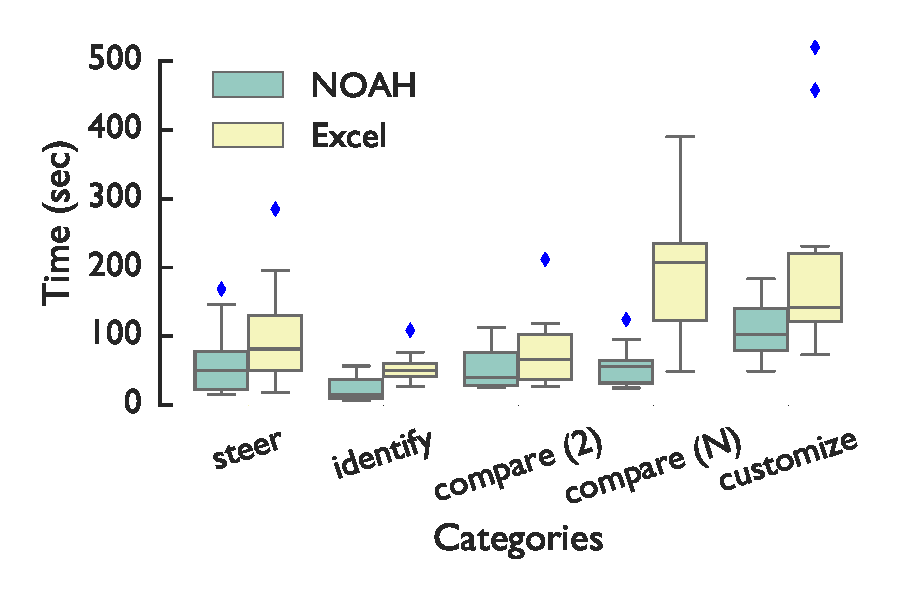
\includegraphics[width=0.23\textwidth,trim={18 20 20 15},clip]{images/bird_box.pdf} &
   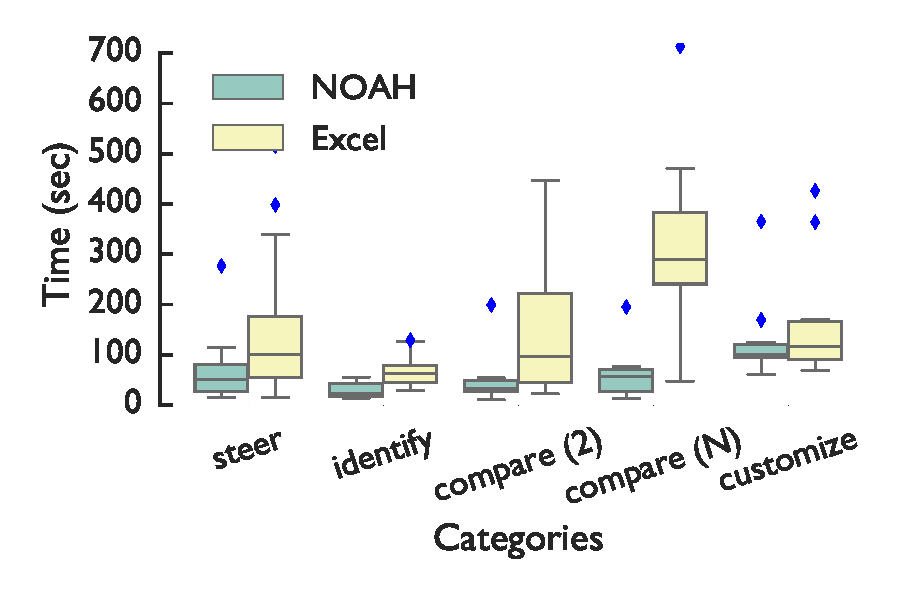
\includegraphics[width=0.23\textwidth,trim={18 20 20 15},clip]{images/airbnb_box.pdf} \\
   \textbf{(a) birdstrikes} & \textbf{(b) airbnb} \\
\end{tabular}
\caption{Submission times per category for each dataset. Median submission times are much smaller for \noah compared to Excel.}
\label{fig:timeBox}
\end{figure}

\subsubsection{Faster navigation without sacrificing accuracy}
\label{sec:time_acc}
In Figure~\ref{fig:timeBox}a and~\ref{fig:timeBox}b, 
we show the distribution of submission times of participants 
for the five task categories, for birdstrikes and Airbnb respectively. 
For most categories, 
\emph{participants' median submission times using \noah 
were less than the fastest submission times using Excel}. This observation suggests that
the new capabilities offered by \noah
made spreadsheet navigation faster for these tasks. \new{We analyzed the intra-participant differences in submission times, which also supported these observations: the majority of submission times using \noah were faster than Excel---19 out of the 20 participants completed at least four tasks in less time using \noah. The submission time differences were more prominent for the steer, find, and \cmpB tasks. \new{In Section~\ref{sec:rq2}, we explain these outcomes in detail. For example, the aggregate column feature provides a faster alternative to steering, the overview-spreadsheet coordination accelerates raw data inspection, and the binned overview coupled with the context bar enables faster comparison.} The differences in submission times were statistically significant for all of the tasks except customize. Both the intra-participant differences and the statistical significance test results are discussed in detail in the Appendix.}

\begin{figure}[!htbt]
   \centering
\begin{tabular}{c c} %trim=left bottom right top
   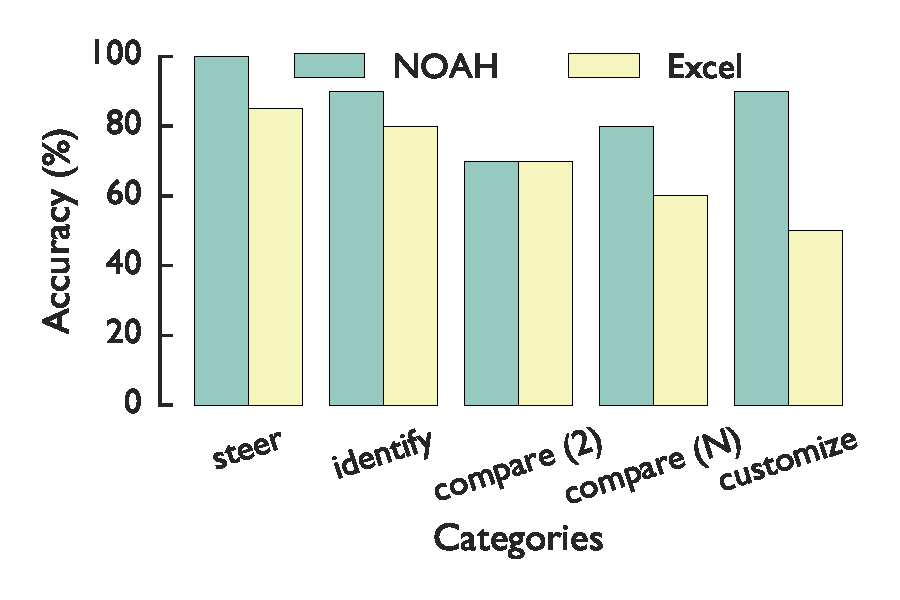
\includegraphics[width=0.23\textwidth,trim={18 20 20 20},clip]{images/bird_accC.pdf} &
   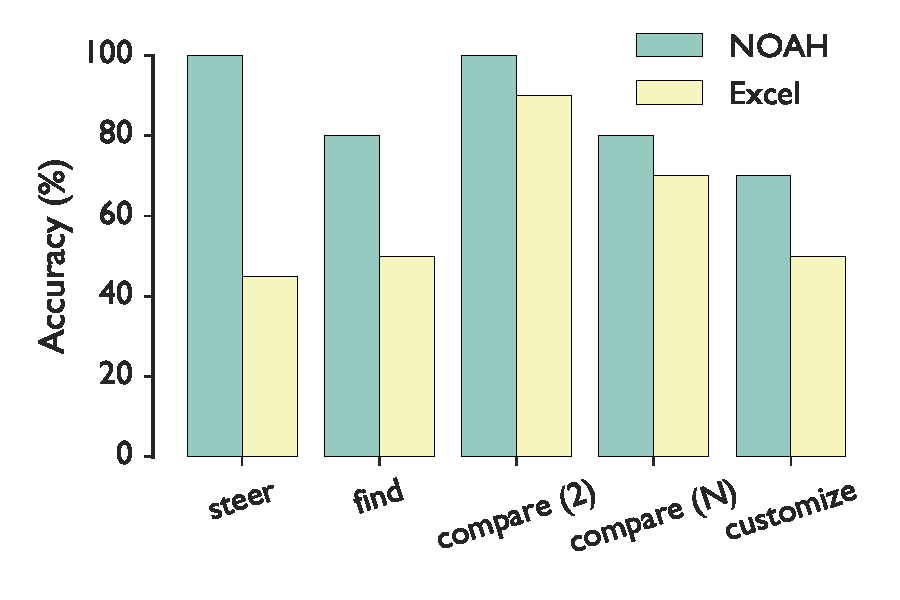
\includegraphics[width=0.23\textwidth,trim={18 20 20 10},clip]{images/airbnb_accC.pdf} \\
   \textbf{(a) birdstrikes} & \textbf{(b) airbnb} \\
\end{tabular}
\caption{Per category accuracy for each dataset. Participants attained higher accuracy while completing tasks in NOAH compared to Excel.}
\label{fig:acc}
\end{figure}
%\subsubsection{Accurate submissions with \noah} 
In Figure~\ref{fig:acc}a and~\ref{fig:acc}b, 
we show the percentage of correct submissions for the four quiz task categories, 
for the birdstrikes and Airbnb datasets, respectively. 
For all the tasks except for the fourth task, \cmpA, for which the accuracy
was the same for both tools, participants 
attained slightly higher accuracy
with \noah compared to Excel. However, the differences in accuracies were statistically significant 
for the steer tasks only (see Appendix). \new{We evaluate the usability of Excel and \noah next.} 
\toappendix{Analysis of screen capture for \cmpA 
revealed that between Florida---the correct answer---and California, 
three participants ($P12$, $P13$, and $P20$) out of 20 
chose the latter when using \noah.}

\begin{figure}[!htbt]
    \centering
    %\vspace{-10pt}
    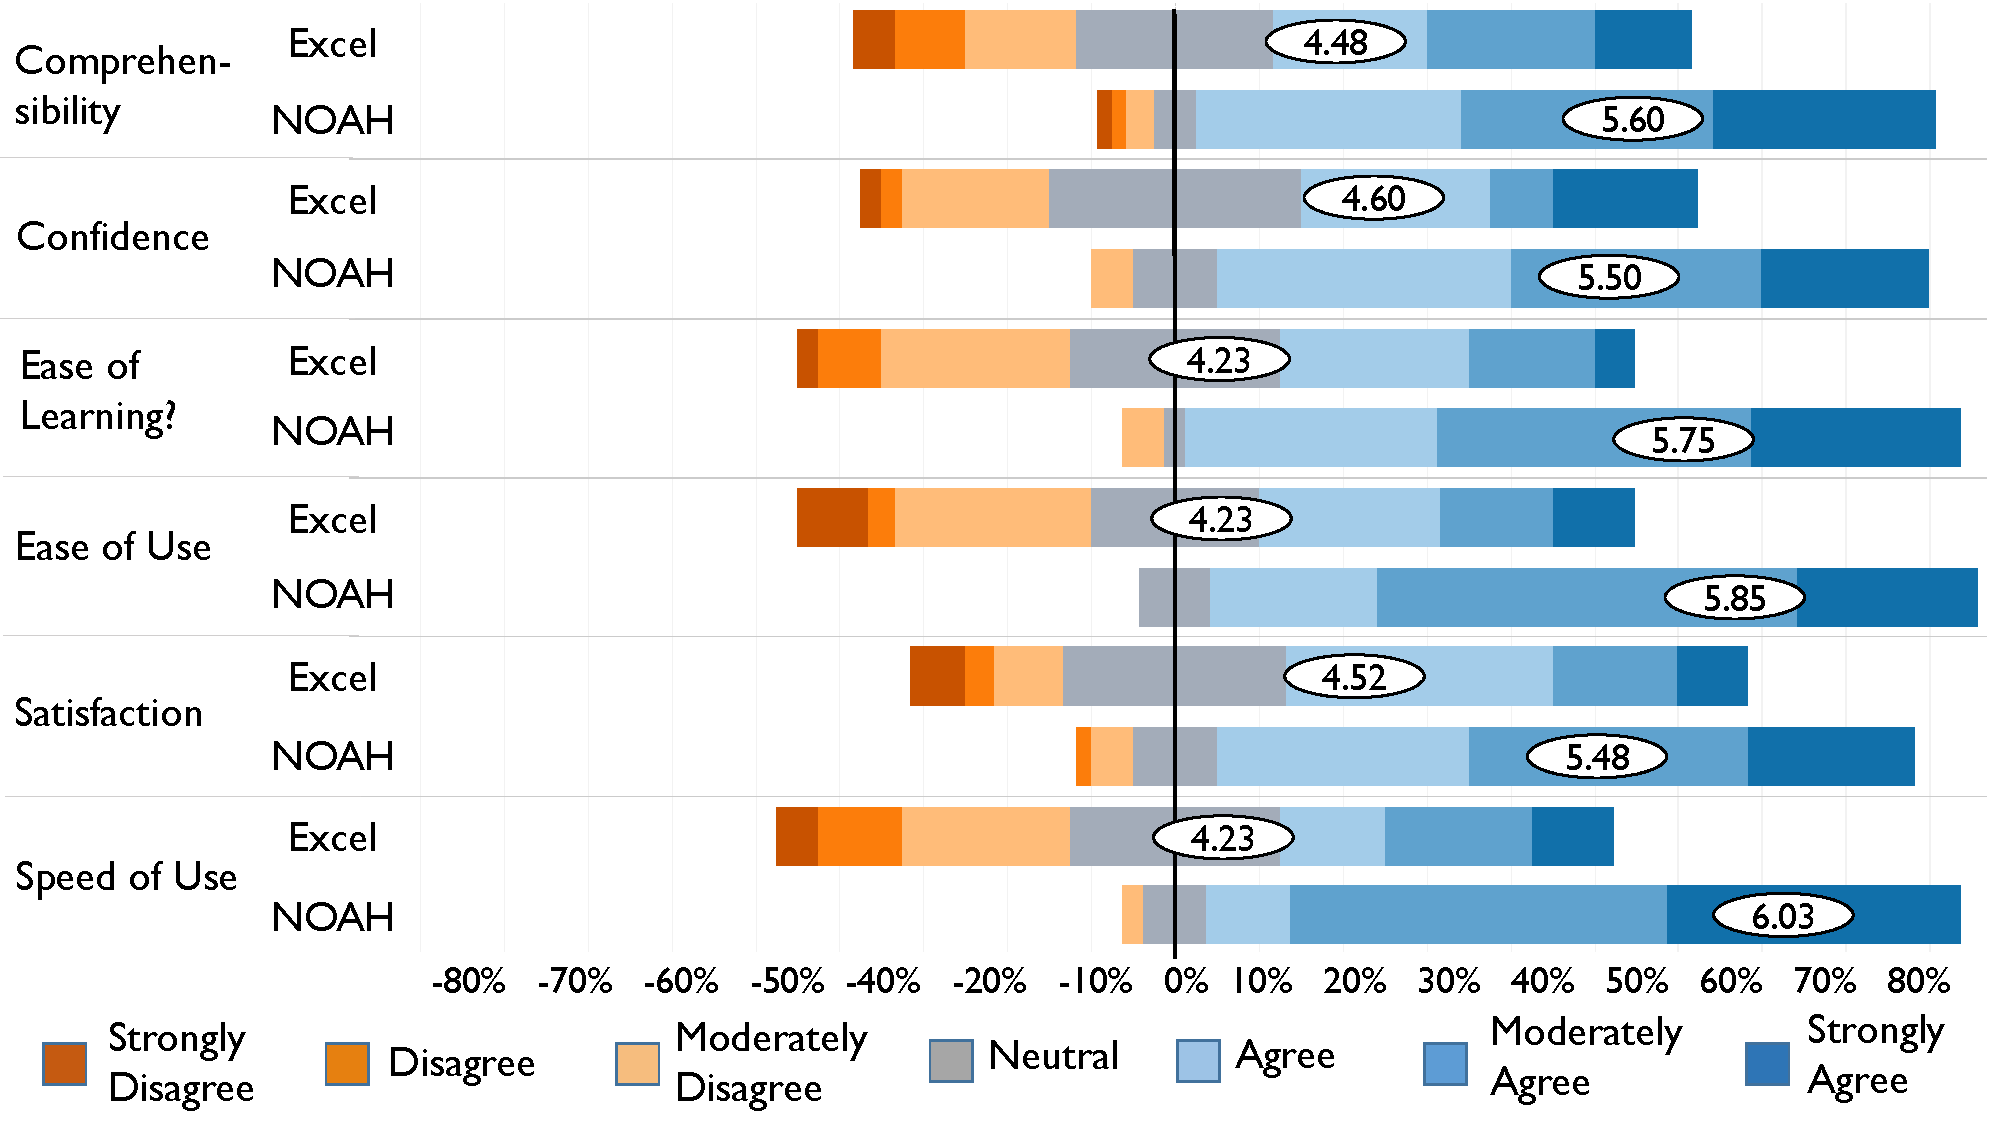
\includegraphics[trim=0 0 0 0,clip,width=\linewidth]{images/survey.pdf}
   \caption{Participants found \noah to be easier to use compared to Excel while being faster in completing tasks involving navigation.}
   \label{fig:survey}
 \end{figure}

\subsubsection{Participants preferred \noah to Excel} 
\new{Figure~\ref{fig:survey} shows a diverging stacked bar chart representation of the survey results in which participants rated their experience with Excel and \noah. 
For each metric mentioned in Section~\ref{sec:study}, there are two stacked bar charts, one for Excel and one for \noah. Each component within a stacked bar represents the percentage of responses for the corresponding rating, where the ratings are on a scale of one one (strong disagreement) to seven (strong agreement). The average rating for each metric is represented with a white ellipse. Notably, \noah had a higher average rating than Excel for all the metrics. The aforementioned observation was further validated by a statistical significance test---the \emph{Wilcoxon Signed-rank Test} (see Appendix). In particular, participants felt that using \noah was faster and easier 
compared to Excel.}
%Even though the features offered by \noah were new to participants they found it fairly easy to learn. 
\toappendix{We further conducted a statistical significance test---the \emph{Wilcoxon Signed-rank} test---on the survey responses which showed that for all the metrics, the ratings significantly differed by the choice of the tool, \ie \noah or Excel. 
The distribution of the ratings for none of the criteria followed a normal distribution.}

\subsection{RQ2. Impact of \noah and its components on spreadsheet navigation experience}
\label{sec:rq2}
\new{To answer RQ2, we assess how \noah's components, \ie the binned overview, aggregate column, and context bar, impacted participants' navigation. For each observation, we present participant feedback from the interview phase.}
%We now discuss how \noah impacted participants' navigation experience compared to Excel.

\subsubsection{Binned Overview: Customizable Hierarchical Organization}
\new{Overall, the binned overview prevented participants from being overwhelmed during navigation, especially at scale. Personalizing the overview enabled participants to define their own grouping of the data, resulting in a more meaningful overview presentation. However, the newer interactions at times deviated from spreadsheet semantics, contributing to a steeper learning curve.}

\stitle{Overviews aid navigation at scale.}
\new{Participants found it difficult to 
perform various navigation tasks in Excel, especially
at scale; \noah, on the other hand, helped participants
avoid endless scrolling via clicking and semantically zooming on the overview, and provided cues for what to explore next via the bins of the overview. 
One participant ($P11$) commented---\response{Excel can get overwhelming 
if you have a lot of data in it and sometimes with that data 
finding things can be difficult}. Participants ($N=6$) mentioned 
that they would prefer \noah when the dataset is large: 
\response{If I just had a large amount of data 
then I would prefer to use \noah because then you 
would be able to see all of it (bins) at once} ($P2$).
\noah's binned overview helped participants comprehend
the overall structure of the data better 
and prioritize the bin they want to visit next. 
One participant ($P5$) commented: 
\response{I think it was just a little bit easier to navigate 
and find where things were because you 
could already see what bins had what.} Another participant ($P1$) said:  
\response{I like \noah a lot better. 
It was a lot easier to look up different data 
and it was a lot quicker too}.}
%Out of 20 participants, 15 preferred \noah for tasks involving navigation. 

\stitle{\new{Overview customization enables related data to be analyzed
together in task-specific ways.}} 
\new{Bin customization enabled participants to 
personalize the overview based on their specific needs. 
One participant ($P16$) commented: 
\response{I did like the fact that it lets you take a data sheet and, in some way, containerize the stuff you care and the stuff you don't care about.} 
Participants (14 out of 20) 
preferred the feature to Excel's filtering feature 
when working with numeric data---\response{That was so much easier in \noah 
than it was in Excel to be able to 
specify the range that you wanted it to go in} ($P17$). 
Our analysis of the video recordings revealed that 
for the birdstrikes dataset in Excel,
the customize task involved filtering out 
certain values from a total of 451 unique values. 
This manual filtering led to a significant delays in
task completion, compared to \noah where they were able to use the bin customization feature. 
However, the time taken for this task was higher than  other tasks in \noah, as
it required participants to restructure the overview
before any calculation could be performed.}

\stitle{\new{Overview customization interactions have a steeper learning curve.}}
\new{Unfamiliarity with the interactions required
during customization in \noah
also contributed to higher 
task completion times for the customize task  
compared to other tasks.
The unfamiliarity led to some participants ($N=5$ out of 20) 
preferring Excel over \noah for this task. 
One participant ($P11$) commented: \response{Since I'm not used to spreadsheet data being presented that way, it took a little bit of getting used to.} Participants found some of the terminology 
used in the interface---\eg explore, bin---quite 
unfamiliar ($N=14$). 
Moreover, two participants didn't understand how the bins were constructed and
requested implementation details during the interview.}

\stitle{\new{Tradeoffs between hierarchical and flat overviews.}}
\new{While participants generally appreciated 
the binned representation of the overview for numeric data, 
a number of participants ($N=6$) stated that they would have preferred a non-hierarchical overview for categorical data, 
where each bin corresponds to one item. One participant ($P13$) commented: \response{I would prefer it start with all the bins split, and then I can merge them as I want.} Another participant ($P4$) said---\response{When I started, it (\noah) had already grouped them, I think, alphabetically. So, that creates an extra step in that I then have to go split them and then re-merge them.}} 

\subsubsection{Aggregate Column: In-situ Steering-free Computation}
\new{The aggregate column feature enabled participants to avoid cumbersome steering interactions, resulting in  faster and more accurate analysis compared to Excel. However, comparing the analysis results of more than two data subsets resulted in increased visual discontinuity and consequent errors.}

\stitle{\new{Cumbersome steering replaced by a few button clicks with aggregate columns.}} 
\new{The steer tasks required participants 
to issue a \code{COUNTIF} formula on a data subset. 
Participants found scrolling and steering in Excel 
to be cumbersome while issuing formulae---\response{The one thing
with Excel is I always try to go to the bottom of the data 
and type in the formula, and with something really long like this, 
the scrolling is a little bit cumbersome} ($P4$). 
With \noah, participants avoided steering by \new{using aggregate column feature on the menu-bar and selecting the appropriate formula}. Multiple participants ($N=13$) found it easier to issue formulae using this feature.
One participant ($P3$) commented: 
\response{And that creates convenience sort of because then you don't have to memorize anything and using the system becomes easier.} 
Another participant ($P13$) commented: \response{There were some formulas to calculate, that were definitely easier in \noah because the aggregate column did all the work and showed me the results.} However, two participants found the aggregation operations 
applied on the bins to be opaque compared to Excel 
where a user can directly manipulate the formula. 
}

\stitle{\new{Issuing formulae is faster and more accurate with aggregate columns.}} 
\new{While the accuracies and submission times for the steer tasks in Excel varied significantly across datasets, using \noah, participants exhibited higher accuracies and faster submission times irrespective of the dataset (see Figure~\ref{fig:timeBox} and~\ref{fig:acc}). The automated and steering-free aggregate column feature of \noah contributed to high accuracies (100$\%$) for the steer tasks.  One participant ($P12$) commented: \response{With \noah, 
you don't have to highlight every number versus Excel where you actually have to select everything.} All of the 14
inaccurate submissions with Excel involved steering an incorrect spreadsheet region; 11 of the inaccurate submissions were with the Airbnb dataset. In \noah, participants were able to avoid steering by using the aggregate column feature. Analysis of screen recordings
revealed that, for Excel, for the birdstrikes dataset, several participants
used the \emph{autosum}
feature to quickly count the number of $1$'s in the binary-valued column involved in the steering task. Summing up
binary values is equal to the number of $1$'s in the collection. 
Other participants used the status bar at the
bottom of the spreadsheet that displayed the sum 
of the cells in the selected column. 
In both cases, participants avoided steering the data resulting in fewer errors. 
On the other hand, for the Airbnb dataset, participants 
could not use these shortcuts as the column involved in the steering task was non-binary 
(it had 365 different values). Failure to avoid steering often led participants
to select an incorrect range of data ($N=14$ cases), resulting in incorrect
responses.  
Therefore, the participants' ability to avoid steering 
depended on the data type.}

\stitle{\new{Visual discontinuity during comparison while reduced, was not completely eliminated.}} 
\new{For \cmpB tasks, participants 
had to perform $N$ comparisons in \noah while issuing the aggregate column operation once. However, the comparison among $N$ bins resulted in increased visual discontinuity. This lead to some ($N=4$ out of 20) incorrect submissions. In Excel, the experience was worse, as the participants had to perform $N$ separate steering tasks. As a result, in Excel, the \cmpB task submission times were very high compared to \cmpA tasks (see  Figure~\ref{fig:timeBox}). In addition, the accuracies of the \cmpB task in Excel were lower ($N=7$ out of 20 submissions were inaccurate).}
\cut{aggregate  column  is  kept  in
sync  with  the  bins  a}

\subsubsection{\new{History, Context, and Coordination}}
\new{The context bar enabled participants to revisit previously explored bins. The aggregation results corresponding to that bin were automatically updated in the aggregate column, due to automatic syncing between the binned overview and aggregate column (see Section~\ref{sec:agg_col}). 
 The coordination between the overview and the raw spreadsheet data further helped participants relate the aggregate column results with the raw data.}

\stitle{\new{History helps avoid repeated interactions.}}
\new{For the \cmpA task in \noah, all of the participants used the context bar to navigate to a bin previously visited for the first steer task. As the bin currently being displayed was changed, the aggregate column was automatically updated to display values corresponding to that bin, enabling participants to view the aggregate column values instantly without having to reissue the operation.} \new{On the other hand, as Excel did not preserve any navigation history, participants had to re-execute the first steering operation. As a result, the submission times for \cmpA tasks were faster in \noah compared to Excel (see Figure~\ref{fig:timeBox}). One participant ($P16$) commented---\response{Once I got familiar with the interface, it was easy to just say, I want to see this state, and I like that fact that like automatically it goes into the bins on NOAH, gave me summary information.} Another participant ($P9$) said---\response{Noah was easy to find and compare and toggle in between.} }

%The completion times were faster in \noahthan in Excel, irrespective of the comparison tasks and datasets. \emph{\noah offers three additionalbenefits apart from avoidance of steering that may have contributed to such improvement}:
%a) participants used the navigation features to access and compare different subsets of data quickly, 
% b) participants did not need to reissue the aggregation formula for any of the bins they navigated to, and 
%c) participants used the value bars presented along with the results in the aggregate column to visually compare different subsets.
%For \cmpB tasks, the number of subsets to be compared was  higher in birdstikes (50) compared to Airbnb (16). As a result, participants exhibited lower accuracy for birdstrikes when using Excel. In \noah, all the participants first split all the bins to create $N$ bins each corresponding to one state. Then participants panned across the overview to find the desired bin as they compared the values. Even in \noah, comparisons between multiple values resulted in increased visual discontinuity leading to some ($N=4$ out of 20) incorrect submissions.
\stitle{\new{Overview-spreadsheet coordination helps relate interactions on the overview with the raw data.}}
\new{The coordination between the overview and spreadsheet in \noah enabled users to quickly relate their interactions on the overview with the raw spreadsheet data. For example, for the find task, 
participants had to find all the cells within the spreadsheet that satisfy a condition corresponding to the preceding steer task.
To do so, they had to
skim through all the cells 
in the current window in Excel, 
resulting in higher completion times.
%Again, participants had to skim over binary values when counting in birdstrikes versus non-binary values for Airbnb, resulting in even higher completion times for the latter. 
Even though Excel supports a conditional formatting feature\footnote{\new{The conditional formatting feature in Excel enables users to request cells that satisfy certain conditions to be colored.}}, issuing the feature added one additional step when performing the find task.} 
\new{In \noah, participants benefited from having visual cues in the form of automatically colored cells, helping them relate the aggregate column with the raw data---\response{You didn't have to do any additional steps and it was a visual cue right there, made it very quick to count it up ($P17$).} Another participant ($P9$) commented---\response{In Excel, you would have to add your own condition for formatting. But you have to build that (conditional formatting) every time  you need to ask a question. This one (\noah) at least something is pre-built in, and you can easily count.} However, one participant ($P3$) pointed out that, when the data corresponding to the bin does not fit in the screen, they had to scroll through to identify relevant information.}
%Out of 20 participants, 16 participants preferred the automatic data highlighting feature of \noah while performing the \emph{identify} task. Moreover, the colored cells focused their attention to relevant regions within the spreadsheet Another participant ($P5$) mentioned the fact that some of the color choices would make \noah unusable for the colorblind population.}
